\model{My Big Integer}

The following class extends the functionality of \java{BigInteger} to allow comma-separated strings (e.g., \java{"123,465,789"}).
The UML diagram summarizes the relationship between the two classes.

\vspace{1em}
\hfill 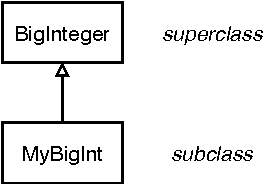
\includegraphics{MyBigInt.pdf} \hspace{2em}
\vspace{-8em}

\begin{javanum}
import java.math.BigInteger;

public class MyBigInt extends BigInteger {

    public MyBigInt(String val) {
        // remove comma characters
        super(val.replace(",",  ""));
    }

    public String toString() {
        // start with the decimal representation
        String str = super.toString();
        StringBuilder sb = new StringBuilder(str);

        // insert comma separators every three digits
        for (int i = sb.length() - 3; i > 0; i -= 3) {
            sb.insert(i, ',');
        }
        return sb.toString();
    }

}
\end{javanum}


\quest{20 min}


\Q Based on the UML diagram:

\setlength{\defaultwidth}{8em}

\begin{enumerate}
\item Which class is the subclass?   \ans{MyBigInt}
\item Which class is the superclass? \ans{BigInteger}
\end{enumerate}


\Q The keyword \java{super} behaves like the keyword \java{this}, except that it refers to the superclass.
On the following lines, which method (in which class) is being invoked?

\setlength{\defaultwidth}{15em}

\begin{enumerate}
\item Line 7:  \ans{constructor in BigInteger}
\item Line 11: \ans{toString in BigInteger}
\item Line 18: \ans{toString in StringBuilder}
\end{enumerate}


\Q Open \textit{MyBigInt.java} in your editor.
Copy the following code snippets into the \java{main} method, one at a time (without the others), and run them.
Record the results in the table below.

\setlength{\defaultwidth}{15em}

\begin{center}
\begin{tabularx}{\linewidth}{|X|p{15.5em}|}
\hline
\multicolumn{1}{|c|}{\tr Java Code} &
\multicolumn{1}{ c|}{\tr Result} \\
\hline

\java{BigInteger bi = new BigInteger("123456789");}
& \\
\java{System.out.println(bi);}
& \ans{123456789} \\
\hline

\java{MyBigInt bi = new MyBigInt("123456789");}
& \\
\java{System.out.println(bi);}
& \ans{123,456,789} \\
\hline

\java{BigInteger bi = new BigInteger("123,456,789");}
& \\
\java{System.out.println(bi);}
& \ans{NumberFormatException} \\
\hline

\java{MyBigInt bi = new MyBigInt("123,456,789");}
& \\
\java{System.out.println(bi);}
& \ans{123,456,789} \\
\hline

\java{BigInteger bi1 = new BigInteger("123456789");}
& \\
\java{MyBigInt bi2 = new MyBigInt("123,456,789");}
& \\
\java{System.out.println(bi1.equals(bi2));}
& \ans{true} \\
\java{System.out.println(bi2.equals(bi1));}
& \ans{true} \\
\hline

\end{tabularx}
\end{center}


\Q Based on the results of the previous question, summarize what the source code for each method does:

\begin{enumerate}

\item \java{MyBigInt} constructor

\begin{answer}[3em]
It first removes any commas from the given string.
It then invokes the constructor of \java{BigInteger} to initialize the object.
\end{answer}

\item \java{MyBigInt.toString}

\begin{answer}[3em]
It first invokes the \java{toString} method of \java{BigInteger}.
It then uses a \java{StringBuilder} to insert commas into the result.
\end{answer}

\item \java{MyBigInt.equals}

\begin{answer}[3em]
It compares the numerical contents of one \java{BigInteger} with another.
(The commas in \java{MyBigInt} are not stored; they are inserted by \java{toString}.)
\end{answer}

\end{enumerate}


\Q \label{key1}
Why do you think \java{bi2.equals(bi1)} compiles and runs correctly, even though the \java{MyBigInt} class does not define an \java{equals} method?

\begin{answer}[3em]
\java{MyBigInt} uses (inherits) the \java{equals} method from \java{BigInteger}.
\end{answer}


\Q \label{count1}
Refer to the \href{https://docs.oracle.com/en/java/javase/11/docs/api/java.base/java/math/BigInteger.html}{documentation for BigInteger} and the source code for \java{MyBigInt}.
How many public items are defined in each class?

\setlength{\defaultwidth}{2em}

\begin{multicols}{2}
\begin{enumerate}
\item \java{BigInteger} fields: \ans{4}
\item \java{BigInteger} constructors: \ans{8}
\item \java{BigInteger} methods: \ans{50}

\item \java{MyBigInt} fields: \ans{0}
\item \java{MyBigInt} constructors: \ans{1}
\item \java{MyBigInt} methods: \ans{1}
\end{enumerate}
\end{multicols}


\Q \label{count2}
Answer each question by typing the following code in \java{main} and pressing \textsf{Ctrl+Space} to list possible completions.

\begin{enumerate}

\item How many public fields does a \java{MyBigInt} have?
\hspace{2.5em} \java{bi2.}
\\ \ans{4} (\textit{Hint:} scroll down to the bottom)

\item How many constructors does a \java{MyBigInt} have?
\hspace{2.5em} \java{bi2 = new MyBigInt(}
\\ \ans{1} (ignore anonymous inner types)

\item About how many methods does a \java{MyBigInt} have?
\hspace{1.3em} \java{bi2.}
\\ \ans{61} (not counting the \java{main} method)

\end{enumerate}


\Q \label{key2}
Notice that \java{MyBigInt} has most of the same fields and methods as \java{BigInteger}.
Non-private fields and methods are \emph{inherited} when extending a class.
Based on your answers to the previous two questions, what is \underline{not} inherited?
Explain your reasoning.

\begin{answer}[3em]
Constructors are not inherited.
\java{BigInteger} has 8 constructors, but \java{MyBigInt} has only 1.
\end{answer}


\Q Make the following changes to \textit{MyBigInt.java}, and summarize the compiler errors.

\begin{enumerate}

\item Rewrite the constructor using two lines of code:

\java{String str = val.replace(",",  "");} \\
\java{super(str);}

\begin{answer}[2em]
Constructor call must be the first statement in a constructor.
\end{answer}

\item Remove all code from the body of the constructor.

\begin{answer}[3em]
Implicit super constructor BigInteger() is undefined.
\\ Must explicitly invoke another constructor.
\end{answer}

\item Remove the constructor altogether.

\begin{answer}[3em]
Implicit super constructor BigInteger() is undefined for default constructor.
\\ Must define an explicit constructor.
\end{answer}

\end{enumerate}
